\chapter{Introduction}
\label{chap:intro}

\section{Charge Transport in Organic Semiconductors}
\subsection{Organic Semiconductors}
Conductive polymers were first discovered in 1977 by Shirakawa et al  \cite{chiang_electrical_1977, Shirakawa1977Jan} for which they were awarded the Nobel prize in Chemistry. Recently these materials have become ubiquitous in many technologies, such as in organic photovoltaic cells\cite{Kippelen2009}, organic field-effect transistors (OFET) \cite{Malachowski2010Jun} and organic light-emitting diodes (OLED) \cite{ThejoKalyani2012Jun}. While the other two technologies lag behind their inorganic counterparts, uptake of OLED screens is becoming ubiquitous -especially in the smartphone and television market due to their flexibility, better colour representation and lower energy consumption than standard backlit LCD displays. OLEDs have also found uses in lighting with their efficiency rivalling that of fluorescent tubes \cite{Reineke2009May, OLED_lighting}. Although, industry has made large strides in fabricating and using these materials the exact nature of the charge transport is still poorly understood. Traditional theories (such as hopping and band transport) aren't applicable to many relevant materials \cite{coropceanu_charge_2007, Giannini2019, C0CS00198H, Fratini_2016, yavuz_dichotomy_2017} as charge transfer dynamics lies in an intermediate region where the polaron is neither fully localised or delocalised. This is due to crystals typically being formed of organic molecules weakly held together by Van der Waals (VDW) forces rather than strong covalent bonds. This allows molecules to fluctuate about their lattice sites and introduces a disorder that doesn't appear in inorganic crystals. 
\\\\
In order to properly quantify the performance of organic semiconductors a key property is the charge carrier mobility. Typically, charge carrier mobilities in `good' organic semiconductors (OSCs) fall between 1-10 cm$^2$V$^{-1}$s$^{-1}$ \cite{Brown2018Mar}. Though higher mobilities, in pure crystals such as Rubrene, have been recorded in the range 15-20+ cm$^2$V$^{-1}$s$^{-1}$ \cite{Zimmerling_RubMob, Podzorov_Rubrene}. This is beyond the range of hopping model validity ($\sim$1 cm$^2$V$^{-1}$s$^{-1}$) and below that of band theory ($>$ 50 cm$^2$V$^{-1}$s$^{-1}$) \cite{yavuz_dichotomy_2017}. In this intermediate regime the charge carriers are typically not completely delocalised at the valence band edges (band regime) or localised to a single site/molecule (hopping regime) but delocalised over a few/tens of molecules \cite{giannini_crossover_2018}. Without any analytic approaches currently being valid in this regime many atomistic computational approaches have been developed to investigate the underlying charge transport mechanisms\cite{oberhofer_charge_2017}.
\\\\
\section{Atomistic Simulations of Nonadiabatic Processes}
In simulating processes involving electronic transfers a key approximation used in conventional molecular dynamics (MD) breaks down. That is the Born-Oppenheimer or adiabatic approximation \cite{john_c._tully_nonadiabatic_nodate}. This approximation, relied upon for almost a century \cite{Pisana2007Feb}, hinges on the fact that nuclei are much more massive than electrons and are approximately stationary with respect to electron movement \cite{Born1927Jan}. This results in nuclear evolution that is governed by a single, adiabatic, potential energy surface. However, in many interesting processes, such as the proton coupled electron transfer in photosynthesis and respiration
 \cite{Hammes-Schiffer2001Apr, Hammes-Schiffer1994Sep, Huynh2007}, non-radiative decay and photochemical processes, electronic transitions between adiabatic potential energy surfaces occur \cite{tully_nonadiabatic_1991}. Simulating these processes requires non-adiabatic molecular dynamics (NAMD) techniques to be developed, to correctly capture dynamical properties.
\\\\
There have been many techniques proposed for use in NAMD such as the quantum classical Louiville equation \cite{Kapral1999May}, multiple spawning \cite{Martnnez*2005Oct} or nonadiabatic Bohmian dynamics \cite{Albareda2014Aug}. However, two of the most popular are trajectory surface hopping \cite{Tully1990Jul} and mean-field approaches \cite{Whetten85}. This is probably due to their relative simplicity to implement, efficiency for large systems and proven efficacy in a wide variety of situations
\cite{Shenvi2011Apr}. In these approaches the general aim is to treat as much of the system as possible with (computationally cheaper) classical mechanics. While handling all necessary parts with quantum mechanics \cite{Coker1995Jan}. In Surface Hopping, Ehrenfest and Coupled-Trajectory Mixed Quantum-Classical molecular dynamics (CTMQC) one treats the nuclear subsystem classically and the electronic one quantum mechanically. The nuclei are normally propagated using a velocity verlet algorithm according to Newton's laws and electrons using a fourth order Runge Kutta algorithm according to the time-dependent Schr\"odinger equation. The wavefunction is normally expanded as a linear combination of adiabatic or diabatic states. The nuclei and electrons can also interact. Taking account of this interaction is where these techniques differ. No one technique is perfect, the issues for surface hopping and Ehrenfest are well documented and have been discussed in detail \cite{SubotnikReview2016, Giovanni_2010_deco, Jaeger_2012_deco, Jain2016, Subotnik_2011_deco}. CTMQC is a fairly new technique and its issues are still mostly unknown. In this document I will discuss CTMQC in depth and present results from my own implementation of it as well as presenting its drawbacks. I will also compare these results to Ehrenfest and Trajectory Surface Hopping (TSH).
\subsection{Surface Hopping and Ehrenfest Dynamics \label{sec:Ehren_SH}}
\begin{wrapfigure}{r}{0.45\textwidth}
  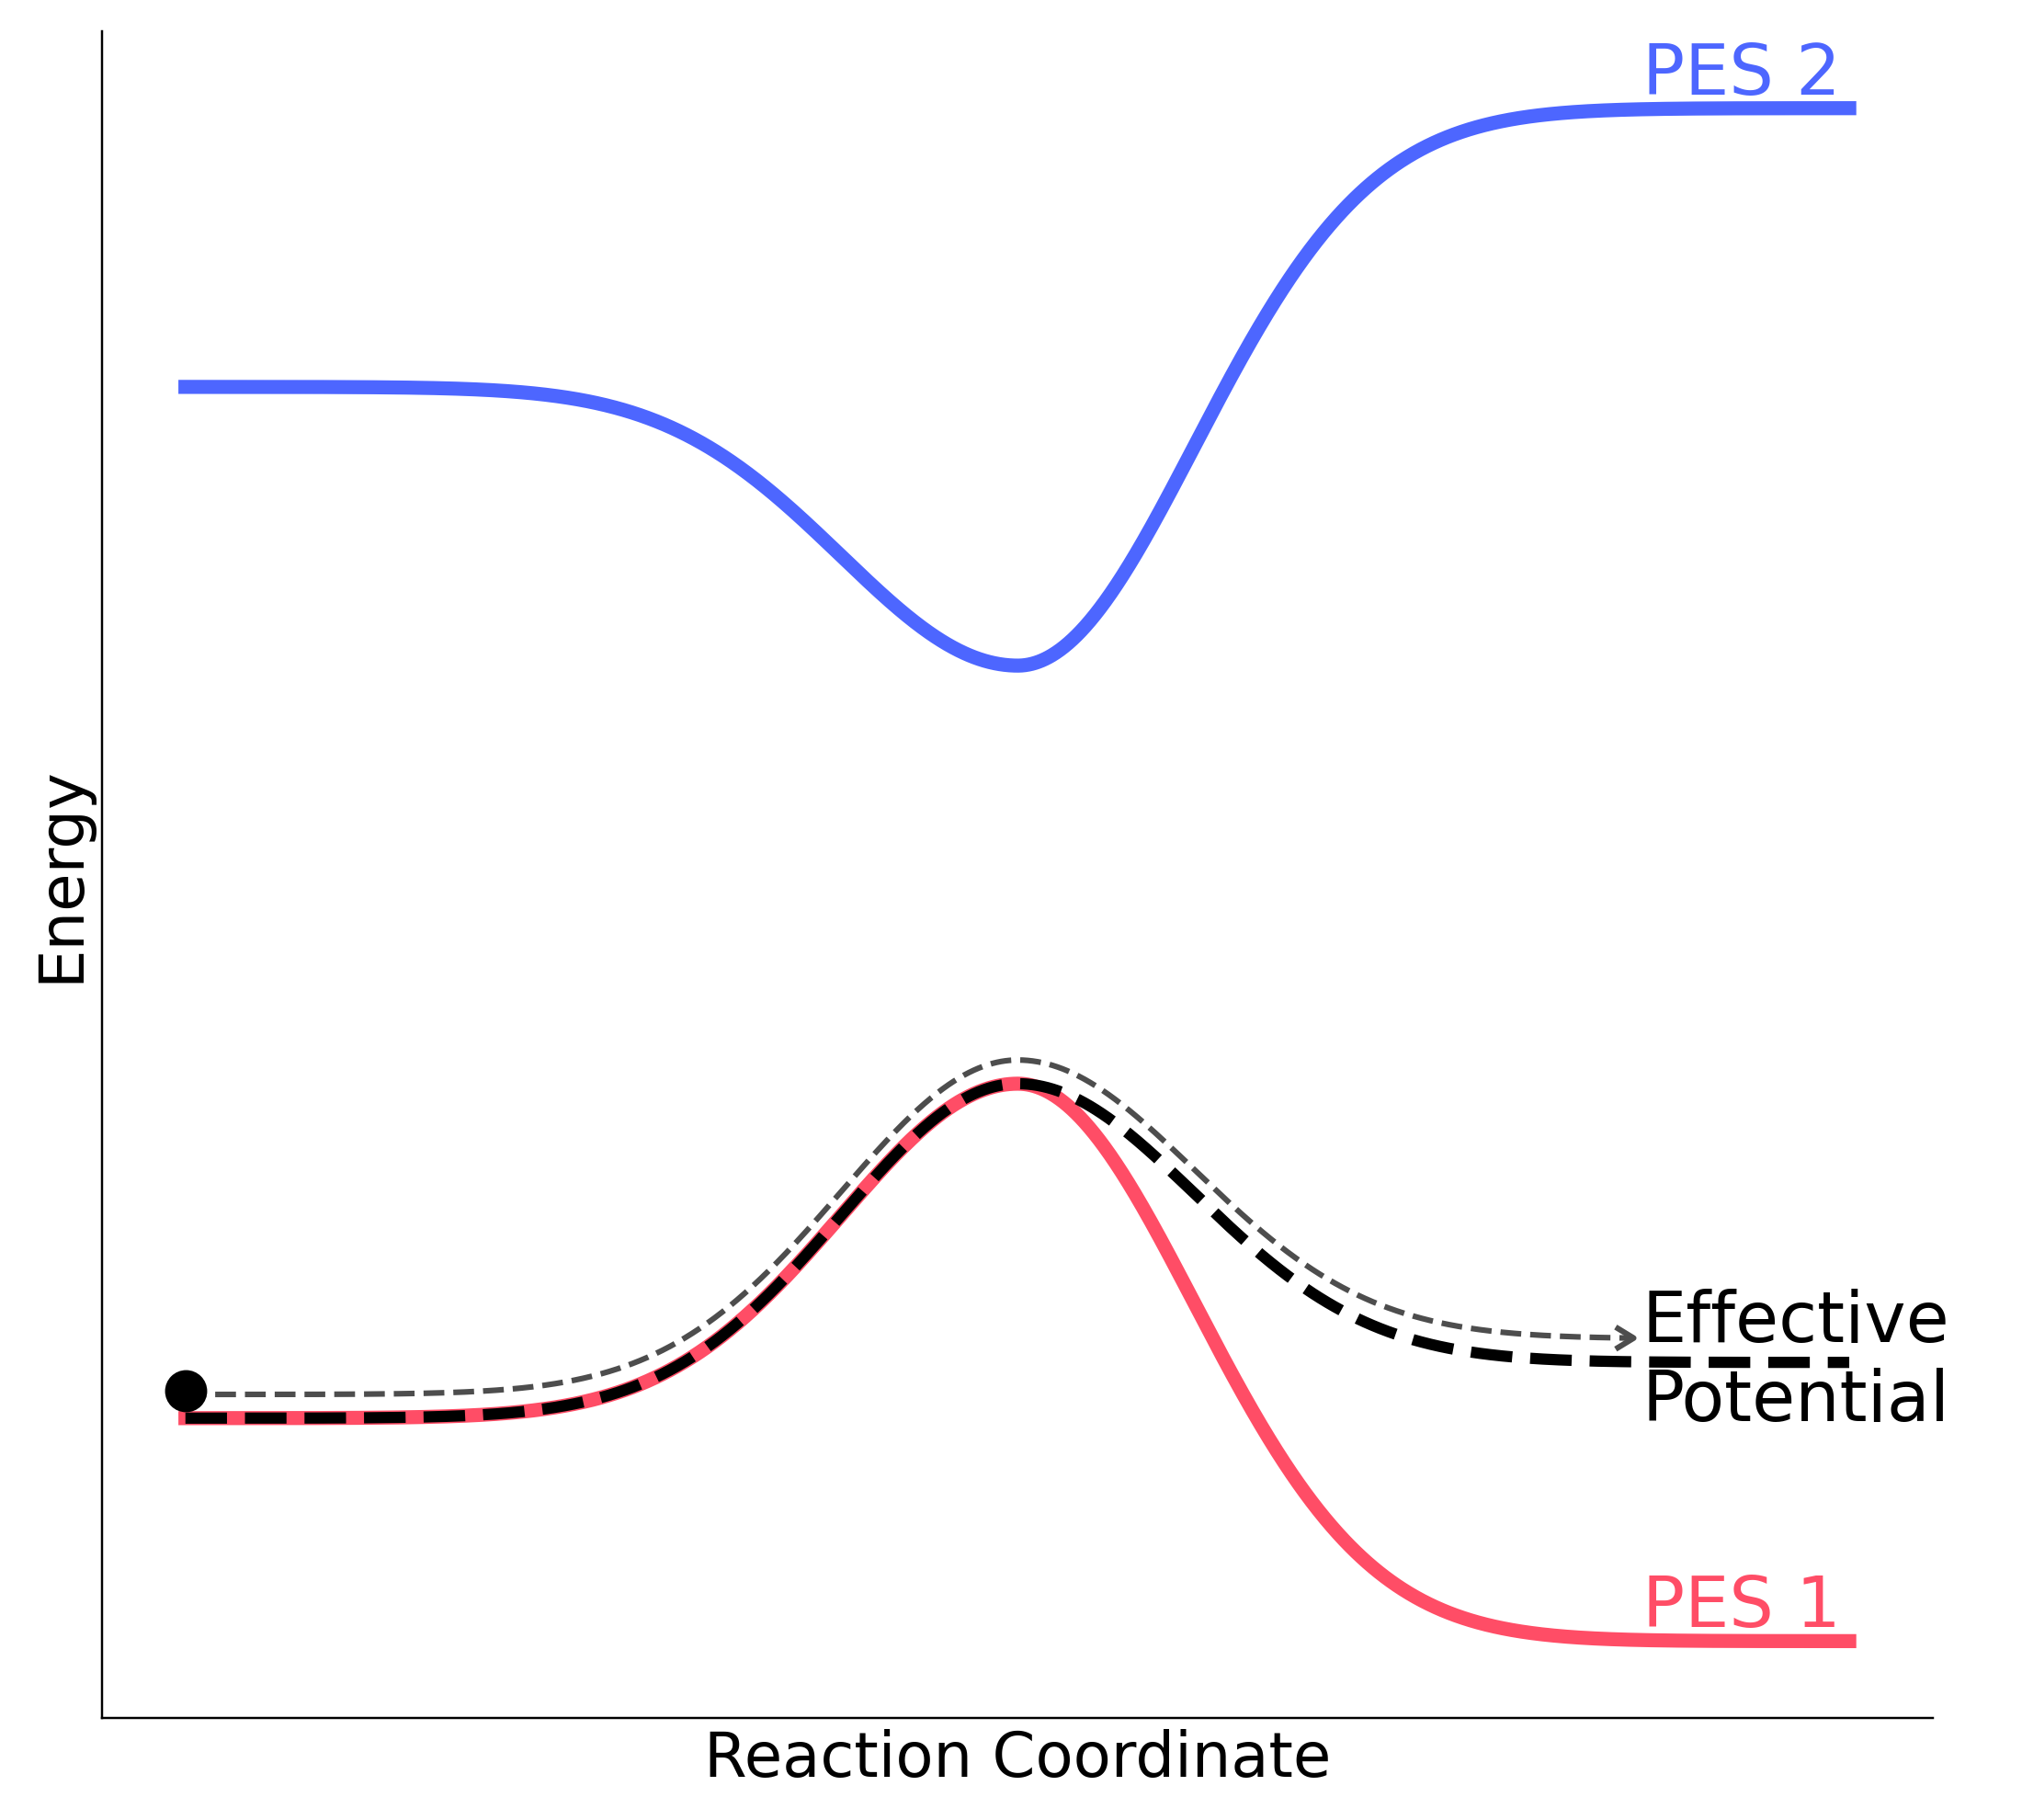
\includegraphics[width=0.45\textwidth]{./img/Eh_hop.png}
  \caption{\label{fig:Eh_diag}An example of a typical Ehrenfest simulation near an avoided crossing. The black lines represent the adiabatic potential energy surface due to the ground (PES 1) and excited (PES 2) state. The red line represents the population weighted average potential the nuclei travel on.}
\end{wrapfigure}
An important technique in the field of mixed quantum classical nonadiabatic molecular dynamics is Ehrenfest dynamics. Assuming we treat the nuclei classically the Ehrenfest equations can be rigorously derived from the electronic Schr\"odinger equation. This is done by assuming that the nuclei's motion is provided by a single population weighted average potential energy surface. This average is taken from the adiabatic potential energy surfaces (eigenvalues of the Hamiltonian) where weights are provided by the populations of each adiabatic state. This effective potential energy surface is shown in fig \ref{fig:Eh_diag}. In this way the electronic subsystem influences the propagation of the nuclei. The propagation of the forces and the electrons are controlled by equations \eqref{eq:Eh_Force} and \eqref{eq:Eh_Elec}.
\\
\begin{equation}
  F_{\nu}^{Ehren} = \sum_i^{N_{st}} |C_{i}|^2 \nabla_{\nu} E_{i} + \sum_{i,j}^{N_{st}} C_{i}^{*} C_{j} (E_{j} - E_{i}) \mathbf{d}_{ij, \nu}
  \label{eq:Eh_Force}
\end{equation}
\begin{equation}
  i \hbar \vec{C}_{m} = C_{m}E_{m} -  i \ \hbar  \sum_{n}^{N_{st}} C_{n} d^{ad}_{mn}
  \label{eq:Eh_Elec}
\end{equation}
In the above equations $C_{i}$ is the adiabatic expansion coefficient for state i, $E_{m}$ is the energy of adiabatic state m, $\mathbf{d}_{mn, \nu}^{ad}$ is the nonadiabatic coupling (in the adiabatic basis) between states m and n for atom $\nu$. The $d_{mn}^{ad}$ are the nonadiabatic coupling elements expressed in the adiabatic basis.
Although the Ehrenfest method has been applied with success in many systems \cite{Li2005Aug, Saita2012Dec, Kohen1998Sep} it has a number of key shortcomings. Namely, its inability to capture the branching of the nuclear wavefunction as propagation occurs on only a single potential energy surface and its poor account of the decoherence of the electronic and nuclear subsystem after an avoided crossing. Ehrenfest also violates detailed balance by populating all adiabatic states evenly \cite{tully_perspective:_2012, john_c._tully_nonadiabatic_nodate}. In the limit of infinite states this results in infinite electronic temperature \cite{parandekar_detailed_2006}.
\begin{wrapfigure}{r}{0.45\textwidth}
  \includegraphics[width=0.45\textwidth]{./img/SH_hop.png}
  \caption{\label{fig:SH_diag}An example of a typical Surface Hopping simulation near an avoided crossing. The black lines represent the adiabatic potential energy surface due to the ground (PES 1) and excited (PES 2) state. The red line represents the discontinuous effective potential the nuclei travel on.}
\end{wrapfigure}
\noindent Possibly the most popular technique in NAMD is trajectory surface hopping. In trajectory surface hopping the shape of the potential energy surface is determined by a series of discrete stochastic hops between adiabatic potential energy surfaces \cite{tully_perspective:_2012}. See fig \ref{fig:SH_diag}.  The probability of these hops is determined by the non-adiabatic coupling between states.
A swarm of trajectories are used and the probability a hop (non-adiabatic coupling) determines how many of these change state. The nuclear dynamics are dictated by the shape of the energy surface they are travelling on. This method can capture the branching of nuclear wavepacket unlike Ehrenfest. However, it still suffers from a number of issues. The original `fewest switches surface hopping' proposed by John Tully suffered from bad overcoherence of the nuclear and electronic subsystems. That is the electronic and nuclear motion was coupled long after the region of high non-adiabatic coupling (crossing region). The fact that the hops are instant leads to discontinuities and methods need to be implemented to fix these such as velocity re-scaling. Finally, perhaps the most important shortcoming is that this technique has not been derived from first principles and cannot be guaranteed to work generally. These problems have lead to a number of other techniques being developed. One of these, CTMQC, will be studied in this thesis and is the semi-classical limit of the exact factorisation of the time-dependent Schr\"odinger equation.
\clearpage
\section{Exact Factorisation}
Exact factorisation \cite{abedi_exact_2010} involves separating the total molecular wavefunction into a nuclear component and electronic component. Where the electronic component is parametrically dependent on the nuclear coordinates, $\mathbf{R}$. This is shown below in eq \eqref{eq:exact_fact} where $\chi$ is the nuclear wavefunction and $\Phi$ is the electronic one.
\begin{equation}
 \Psi(\mathbf{R}, \mathbf{r}, t) = \Phi_{\mathbf{R}}(\mathbf{r}, t) \chi(\mathbf{R}, t)
 \label{eq:exact_fact}
 \end{equation}
In the above equation (and throughout this report) I will denote nuclear coordinates and electronic coordinates $R$ and $r$ respectively. The nuclear and electronic wavefunctions then obey separate, but coupled, time-dependent Schr\"odinger equations for spatial and temporal evolution. In this report, I will be focussing on the semi-classical limit of these equations, named Coupled-Trajectory Mixed Quantum-Classical Molecular Dynamics (CTMQC), and give results of a combination of this and the AOM method explained in section \ref{ap:FOB}.
\\\\
The equations for the evolution of the electronic and nuclear wavefunctions in the exact factorisation \cite{abedi_exact_2010} are given below:
\begin{align}
  i\hbar \frac{\delta}{\delta t} \Phi_{\mathbf{R}}(\mathbf{r}, t) &= \left( \hat{H}_{BO} + \hat{U}_{en}\left[ \Phi_{\mathbf{R}}, \chi\right] - \epsilon(\mathbf{R}, t) \right) \Phi_{\mathbf{R}} (\mathbf{r}, t)
  \label{eq:electronic_exact}
\\
i\hbar \frac{\delta}{\delta t} \chi (\mathbf{R}, t) &= \left( \sum_{\nu = 1}^{N_{n}} \frac{[-i\hbar\nabla_{\nu} + \mathbf{A}_{\nu}(\mathbf{R}, t)]^2}{2 M_{\nu}} + \epsilon(\mathbf{R}, t)\right) \chi (\mathbf{R}, t)
  \label{eq:nuclear_exact}
\end{align}
Where $\hat{H}_{BO}$ is the Born-Oppenheimer Hamiltonian, that is $\hat{T}_{e} + \hat{W}_{ee} + \hat{W}_{nn} + \hat{V}_{en}$. Where $\hat{T}_{e}$ is the electronic kinetic energy operator, $\hat{W}_{ee/nn}$ is the electron-electron/nuclei-nuclei interaction and $V_{en}$ is the electronic-nuclear potential.
\\\\
The $\hat{U}_{en}$ is an electronic-nuclear coupling operator (ENCO). This is defined as \begin{equation}
  \hat{U}_{en}[\Phi_{\mathbf{R}}, \chi] = \sum_{\nu=1}^{N_{nuc}} \frac{1}{M_{\nu}} \left[ \frac{\left[-i \hbar \nabla_{\nu} - \mathbf{A}_{\nu}(\mathbf{R}, t) \right]^2}{2} + \left( \left. \left. \frac{-i\hbar \nabla_{\nu} \chi}{\chi} + \mathbf{A}_{\nu}(\mathbf{R, t})\right)\right( -i\hbar\nabla_{\nu} -            \mathbf{A}_{\nu}(\mathbf{R}, t)\right) \right]
  \label{eq:ENCO}
\end{equation}
\\
Where the $\mathbf{A}_{\nu}$ is a time-dependent vector potential (TDVP), given by $\left\langle \Phi_{\mathbf{R}}(t) \right\vert \left. - i \hbar \nabla_{\nu} \Phi_{\mathbf{R}} \right\rangle_{\mathbf{r}}$ and $M_{\nu}$ is the mass of nuclei $\nu$.
Finally $\epsilon(\mathbf{R}, t)$ is a time-dependent scalar potential energy surface (TDPES), given by $\langle \Phi_{\mathbf{R}}(t) \vert \hat{H}_{BO} + \hat{U}_{en}^{coup} - i\hbar \frac{\delta}{\delta t} \vert \Phi_{\mathbf{R}}(t) \rangle_{\mathbf{r}}$.
\\
\begin{wrapfigure}{r}{0.5 \textwidth}
  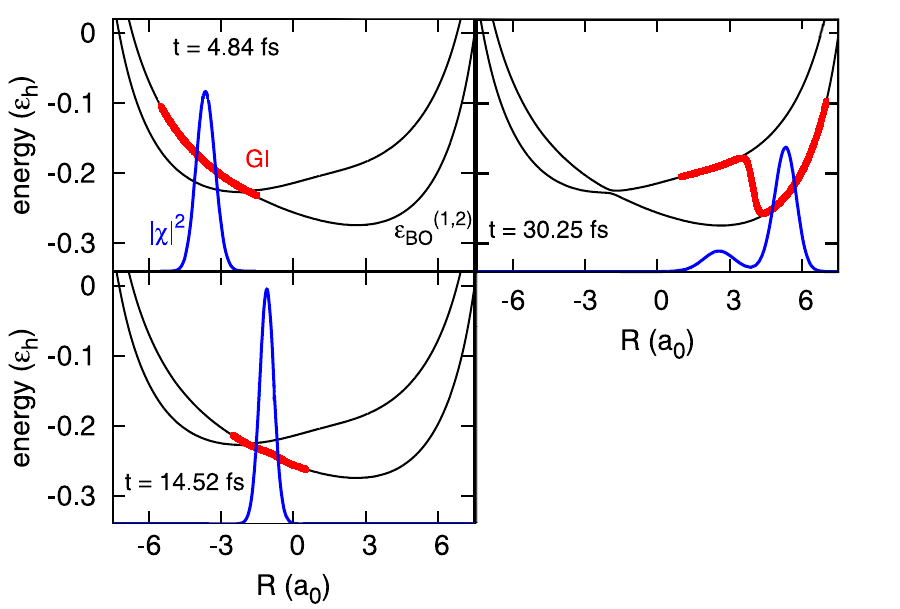
\includegraphics[width=0.5\textwidth]{./img/CTMQC/nuclear_splitting_TDPES.png}
  \caption{A demonstration of how the TDPES can cause the splitting of the nuclear wavepacket in non-adiabatic regions. The red line represents the TDPES and the blue is the nuclear density. Figure adapted from Agostini, 15 \cite{agostini_exact_2015} \label{fig:step_TDPES}}
\end{wrapfigure}
The effects of the TDPES, TDVP and the ENCO have been investigated in multiple works \cite{agostini_semiclassical_2015, agostini_exact_2015, agostini_mixed_2013, abedi_dynamical_2013, Min2014Dec}. The TDPES and TDVP are both responsible for the evolution of the system
\cite{agostini_semiclassical_2015}. The TDPES provides exact classical forces on the nuclei. In fact, an alternative independent-trajectory semi-classical scheme has been investigated using these exact forces \cite{agostini_exact_2015}. This found the TDPES is responsible for the splitting of the nuclear wavepacket in regions of high non-adiabaticity by taking the shape of a step function between the 2 adiabatic potentials. This is demonstrated in figure \ref{fig:step_TDPES}, which was adapted from an image in Agostini, 15 \cite{agostini_semiclassical_2015}. 
\\\\ 
Finally the electronic-nuclear coupling operator (ENCO) is responsible for other non-adiabatic effects in the system such as electronic nonadiabatic transitions and decoherence \cite{agostini_semiclassical_2015}.
\section{Approximations leading to CTMQC}
\label{sect:CTMQC_Approx}
Starting from the exact factorisation equations, 6 approximations have been made to derive the CTMQC equations. These are discussed in detail in Ref. \cite{agostini_quantum-classical_2016}. In the interest of completeness I have summarised them below.
\subsection{Classical Nuclei}
Techniques that include nuclear quantum effects (NQEs); such as multiple spawning \cite{Martnnez*2005Oct}, ring-polymer surface hopping \cite{Shakib2017Jul} and nonadiabatic Bohmian dynamics \cite{Curchod2011Feb, Tavernelli2013Apr} although extremely accurate, cannot be applied to hundreds or thousands of molecules, due to their high computational cost. Further, in many systems of interest NQEs are negligible, especially at room temperature. For this reason the classical limit of the nuclear Schr\"odinger equation \eqref{eq:nuclear_exact} is taken when deriving the CTMQC equations.
\subsection{Neglect the ENCO in the TDPES}
The electron-nuclei coupling operator is omitted in the expression for the time-dependent potential energy surface. This is justified as the first term ($\left[-i \hbar \nabla_{\nu} - \mathbf{A}_{\nu}(\mathbf{R}, t) \right]^2$) contains a second order derivative which is expensive to calculate and has a neglible effect compared to the second term in the ENCO \cite{Scherrer2015Aug}. However, the rest of the ENCO is equal to zero when averaged over $\Phi_{\mathbf{R}}(\mathbf{r},t)$ so it does not contribute to the TDPES.
\subsection{Derivative of the Adiabatic Coefficients}
The derivative of the adiabatic coefficients appears in the electronic evolution equations. However, we can re-write the derivative of the adiabatic coefficients in terms of their modulus and phase:
\begin{equation}
  \nabla_{\nu} C_{l}^{(I)}(t) = \left[ \underbrace{\frac{\nabla_{\nu} |C_{l}^{(I)}(t)|}{|C_{l}^{(I)}(t)|}}_{(\text{Term 1})} + \underbrace{\frac{i}{\hbar} \nabla_{\nu} \gamma_{l}^{(I)}(t)}_{(\text{Term 2})}\right] C_{l}^{(I)}(t)
\end{equation}
It has been found that the first term is negligible compared to the second \cite{abedi_dynamical_2013, agostini_mixed_2013, agostini_exact_2015} so it doesn't need to be calculated and we can remove it. It was also assumed that the NACVs are localised in space meaning that, after some algebra, the spatial derivative of the adiabatic coefficient can be written as:
\begin{equation}
  \nabla_{\nu} C_{l}^{(I)}(t) = \frac{i}{\hbar} \nabla_{\nu} \gamma_{l}^{(I)}(t) C_{l}^{(I)}(t) = -\frac{i}{\hbar} \int^{t} dt' \nabla_{\nu} \epsilon_{l}^{(I)} C_{l}^{(I)}(t) = -\frac{i}{\hbar} \mathbf{f}_{l}^{(I)} C_{l}^{(I)}(t)
  \label{eq:hist_force}
\end{equation}
Where $\epsilon_{l}^{(I)}$ is the energy of the l$^{th}$ adiabatic potential energy surface for trajectory I, $C_{l}^{(I)}$ is the adiabatic expansion coefficient for state l and trajectory I. The $\mathbf{f}_{l}^{(I)}$ is the time-integrated adiabatic force (adiabatic momentum).
\subsection{Gaussian Nuclear Wavepackets}
In order to calculate the quantum momentum -the new term in CTMQC. Knowledge of the nuclear distribution is needed. However, as we treat the nuclei as point particles we need to re-construct the nuclear density from the atomic positions. This is done by smoothing out the atomic positions by placing a gaussian of width $\sigma$ centered on each atomic position and combining these gaussians to produce the final nuclear density. This introduces an empirical parameter ($\sigma$) which will be discussed later in this thesis. It should be noted, the nuclei are still propagated classically, the width parameter is only used in the calculation of the quantum momentum.
\subsection{Seperating the Effects of Decoherence and NACVs}
So as to not introduce any population transfer (due to the quantum momentum) when the NACV is zero a fifth approximation has been introduced. Namely the quantum momentum depends on pairs of states -l,k. This enables the separation of the `competing' effects of the NACV and the Quantum Momentum.
\section{The CTMQC equations}
\subsection{Adiabatic Basis}
\label{sec:ad_eqns}
The equations for the propagation of the classical nuclei and the expansion coefficients in the CTMQC framework in the adiabatic basis are given below:
\begin{dmath}
  \dot{\mathbf{P}}_{\nu}^{(I)} =
  -\overbrace{
     \sum_{k} |C_{k}^{(I)}|^2 \nabla_{\nu}\epsilon_{k}^{(I)}
     - \sum_{k,l} C_{l}^{(I)} C_{k}^{* (I)} \left(\epsilon_{k}^{(I)}  - \epsilon_{l}^{(I)}   \right)
  }^{\text{Ehrenfest}}
  \\
  \underbrace{
    - \sum_{l,k} |C_{l}^{(I)}|^2 \left( \sum_{\nu'=1}^{N_n}    \frac{2}{\hbar M_{\nu'}} \mathcal{Q}_{lk, \nu}^{(I)} \cdot    \mathbf{f}_{l, \nu}^{(I)} \right)\left[ |C_{k}^{(I)}|^2    \mathbf{f}_{k,\nu}^{(I)} - \mathbf{f}_{l,\nu}^{(I)} \right]
  }_{\text{Quantum Momentum}}
    \label{eq:nuc_adiab}
\end{dmath}

\begin{dmath}
  \dot{C}_{l}^{(I)} =
  \overbrace{
    -\frac{i}{\hbar} \epsilon_l^{(I)} C_{l}
    - \sum_k C_k^{(I)} d_{lk}^{ad \ (I)}
  }^{\text{Ehrenfest}}
  \\
  \underbrace{
    - \sum_{\nu=1}^{N_n}\sum_{k} \frac{\mathcal{Q}_{lk, \nu}^{(I)}}{\hbar M_\nu} \cdot \left[ \mathbf{f}_{k,\nu}^{(I)} - \mathbf{f}_{l,\nu}^{(I)} \right] |C_{k}^{(I)}|^2 C_{l}^{(I)}
  }_{\text{Quantum Momentum}}
  \label{eq:elec_adiab}
\end{dmath}
Where the $\epsilon_k$ term is the potential energy on the k$^{th}$ potential energy surface. $C_l$ is the adiabatic expansion coefficient corresponding to the l$^{th}$ state. The sum over k and l indicates a sum over all states, the (I) superscript is a replica index and the $\nu$ is an atom index. $M_{\nu}$ is  the nuclear mass and $d_{lk}^{ad (I)}$ represents the non-adiabatic coupling element (in the adiabatic basis) between adiabatic states l and k.
The 2 new terms in this scheme not seen in other NAMD methods are the $\mathcal{Q}_{lk, \nu}^{(I)}$ and the $\mathbf{f}_{k, \nu}^{(I)}$. These are the quantum momentum and the adiabatic momentum. The adiabatic momentum term is defined in equation \eqref{eq:hist_force} this keeps a record of the previous forces on each adiabatic state in the system. The quantum momentum term couples the trajectories together (making this a coupled-trajectory scheme). Together the history dependent force and quantum momentum are responsible for the decoherence in the `Quantum Momentum' parts of the above equations \cite{gossel_coupled-trajectory_2018}. Notably, although these equations have been derived from the exact factorisation equations separately from Ehrenfest they do contain the Ehrenfest equations within them (marked `Ehrenfest'). This scheme can therefore be seen as an Ehrenfest scheme with a correction that captures branching of the nuclear wavefunction and decoherence within it.
\\\\
We can also see in equation \eqref{eq:elec_adiab} if we are in a pure adiabatic state i.e. all population on a single adiabatic state, there is no contribution from the quantum momentum part of the equations. In this scenario the evolution equations become simply Ehrenfest equations. For example, if all the population is localised on a single adiabatic state then the term $|C_{k}^{(I)}|^2 C_{l}$ is only non-zero when $l = k$. However, when $l = k$, the term $\left[ \mathbf{f}_{k,\nu}^{(I)} - \mathbf{f}_{l,\nu}^{(I)} \right]$ is zero as $\mathbf{f}_{k,\nu}^{(I)} = \mathbf{f}_{l,\nu}^{(I)}$.
Therefore, the quantum momentum term can be seen to only kick in when there is a mixing of adiabatic states. In the adiabatic formulation of these equations it is the adiabatic NACV $\mathbf{d}_{lk, \nu}^{ad, (I)}$ that is responsible for the initial mixing of the populations from pure adiabatic states.
 \section{Calculating the Quantum Momentum \label{sec:calc_QM}}
 \label{sect:QM_Calc}
 The technique for calculating the quantum momentum term is outlined in detail in the SI of min, 17 \cite{min_ab_2017}. The original equations given in Agostini, 16\cite{agostini_quantum-classical_2016} present a quantum momentum term without state indices (l,k). This, due to approximations made in the derivation of CTMQC, results in population transfer even when the non-adiabatic couplings between states are zero. Therefore, Agostini et al enforced this condition with the pair-wise state dependence on the quantum momentum. The quantum momentum is defined in equation \eqref{eq:QM_def} as:
\begin{equation}
  \mathcal{Q}_{\nu}^{(I)} = \frac{-\hbar \nabla_{\nu} |\chi^{(I)}|}{|\chi^{(I)}|} \frac{-\hbar \nabla_{\nu}                            |\chi^{(I)}|^2}{2|\chi^{(I)}|^2}
  \label{eq:QM_def}
\end{equation}
In order to reconstruct the nuclear density, Gaussian distributions are used as in equation \eqref{eq:NuclDens} below:
\begin{equation}
	|\chi^{(I)}(t)|^2 = \frac{1}{N_{tr}} \sum_{J=1}^{N_{tr}} \prod_{\nu=1}^{N_n} g_{\sigma_{\nu}^{(J)}(t)} \left(\mathbf{R}_{\nu}^{(I)}(t) - \mathbf{R}_{\nu}^{(J)}(t)\right)
	\label{eq:NuclDens}
\end{equation}
Where, $N_{tr}$ is the number of trajectories, $N_{n}$ is the number of atoms, $\sigma_{\nu}^{(J)}(t)$ is a time-dependent width parameter for each gaussian $g$ and $\mathbf{R}_{\nu}^{(J)}$ represents the atomic position of atom $\nu$ on trajectory $J$.
\\\\
This results in a linear expression for the quantum momentum.
The full details of the derivation are given in the supplementary information of Min, 17 \cite{min_ab_2017}. The resulting linear expression for the quantum momentum is given below:
\begin{equation}
  \mathcal{Q}_{lk, \nu}^{(I)} = \alpha_{\nu}^{(I)} \mathbf{R}_{\nu}^{(I)} - \mathbf{R}_{lk, \nu}
  \label{eq:QM_lin}
\end{equation}
Where $\mathbf{R}_{\nu}^{(I)}$ are the nuclear coordinates on trajectory I on atom $\nu$. The $\alpha_{\nu}^{(I)}$ term is a weighted  average over trajectories of the product of the gaussian's assigned to each atomic coordinate, i.e:
\begin{equation}
  \alpha_{\nu}^{(I)} = \sum_{J}^{N_{tr}} \frac{\hbar \prod_{\nu'} g_{\sigma_{\nu'}^{(J)}(t)}\left(\mathbf{R}_{\nu'}^{(I)}(t) -         \mathbf{R}_{\nu'}^{(J)}(t)\right)}   {2 \sigma_{\nu}^{(J)}(t)^2\sum_{K}^{N_{tr}}\prod_{\nu'}                                           g_{\sigma_{\nu'}^{(K)}(t)}\left(\mathbf{R}_{\nu'}^{(I)}(t) - \mathbf{R}_{\nu'}^{K)}(t)\right)}
  \label{eq:alpha}
\end{equation}
Along with the $\mathbf{R}_{lk, \nu}$ term the $\alpha_{\nu}^{(I)}$ performs the job of coupling the trajectories together. The $\mathbf{R}_{lk, \nu}$ term also given in the SI of Min, 17\cite{min_ab_2017} is defined for each Cartesian dimension as:
\begin{equation}
  R_{lk, \nu} = \sum_{I}^{N_{tr}} R_{\nu}^{(I)}(t) \alpha_{\nu}^{(I)}(t) \frac{|C_{k}^{(I)}(t)|^2 |C_{l}^{(I)}(t)|^2 \left( f_{k,      \nu}^{(I)}(t) - f_{l, \nu}^{(I)}(t) \right)}{\sum_{J} |C_{k}^{(J)}(t)|^2 |C_{l}^{(J)}(t)|^2 \left( f_{k, \nu}^{(J)}(t) - f_{l,         \nu}^{(J)}(t) \right)}
  \label{eq:Rlk}
\end{equation}
Where the bold notation for vectors has been replaced by normal font. This means that this equation applies to each Cartesian dimension independently. Further, in this expression $R_{lk, \nu}$ is symmetric, $R_{lk} = R_{kl}$ meaning that $Q_{lk} = Q_{kl}$. It is also undefined on the diagonals as the denominator is 0, diagonal values are therefore set to 0. At first sight, the $R_{lk}$ term seems to be another weighted average. However, this isn't quite the case as the denominator can be negative. This causes equation \eqref{eq:Rlk} to be very sensitive to errors in the calculation of the denominator of this fraction. Any inaccuracies can lead to the denominator approaching zero faster than the numerator causing large spikes in the quantum momentum term. This will be discussed in greater detail in the following chapters.


